\documentclass[leqno]{jsarticle}
\usepackage{amssymb}
\usepackage{amsthm}
\usepackage{amsmath}
\usepackage{comment}
\usepackage[dvipdfmx]{graphicx}
%定理環境 thmはあまり使わずpropをなるべく使う。
%主張は基本的に証明の中で使い、そのため番号を付けない。
%注意環境を付けてみた。
\newtheorem{thm}{定理}
\newtheorem{prop}[thm]{命題}
\newtheorem{cor}[thm]{系}
\newtheorem{lem}[thm]{補題}
\newtheorem{df}[thm]{定義}
\newtheorem{exam}[thm]{例}
\newtheorem{fact}[thm]{事実}
\newtheorem*{claim}{主張}
\newtheorem*{cau}{注意}
\renewcommand{\proofname}{{\bf 証明}}
%矢印たち。
%\toは\rightarrowと同じ。\getsは\leftarrowと同じ。同値は\iff
%上向き矢はuparrow逆はdownarrow
\newcommand{\To}{\Longrightarrow}
\newcommand{\Gets}{\LongLeftarrow}
%黒板太字
\newcommand{\nn}{\mathbb{N}}
\newcommand{\zz}{\mathbb{Z}}
\newcommand{\qq}{\mathbb{Q}}
\newcommand{\rr}{\mathbb{R}}
\newcommand{\cc}{\mathbb{C}}
%無限大
\newcommand{\mgn}{\infty}
%差集合は\setminusで統一する。等号の否定は\neq
%真部分集合は\subsetneqq　偏微分は\partial
%ディスプレイスタイル。\dfracでディスプレイ分数
\newcommand{\dpst}{\displaystyle}
\newcommand{\ep}{\varepsilon}
\newcommand{\al}{\alpha}
\renewcommand{\o}{\omega}

%空集合は\Oを使う！！！！！！！！！！！！

\title{コンパクト集合の共通部分}
\author{電波通信}
\date{\today}
			\begin{document}
\maketitle
この文書では２つのコンパクト部分集合の共通部分がコンパクトでないようなものが存在する位相空間を構成する。案外簡単にできるので、この文書を読む前に自分で頑張って構成しようと試みることを推奨する。

以下そのような位相空間を構成する。

$(A,\mathfrak{A})$をノンコンパクトな位相空間とする。$\mathfrak{A}$はこの位相空間の開集合系である。このとき$A$に属さない異なる二元$\al,\o$を与え
\[
X=A\cup \{\al,\o\},\ K=A\cup \{\al\},\ L=A\cup\{\o\}
\]
と置く。さて$X$の部分集合族$\mathfrak{O}$を
\[
\mathfrak{O}=\mathfrak{A}\cup \{X,K,L\}
\]
とする。
このとき$\mathfrak{O}$は開集合系の公理を充たすことは簡単にわかる。更にこの$(X,\mathfrak{O})$の部分空間としての$A$は$(A,\mathfrak{A})$である。さて$K,L$はこの空間$(X,\mathfrak{O})$のコンパクト集合である。なぜなら$K$について言うと$\al$を元に持つ開集合は$X,K$のみだからである。$L$についても同様。そして
$K\cap L=A$
であり、$A$はノンコンパクトであるから、２つのコンパクト集合の共通部分がコンパクトでない空間が得られた。
\begin{figure}[h]
\begin{center}
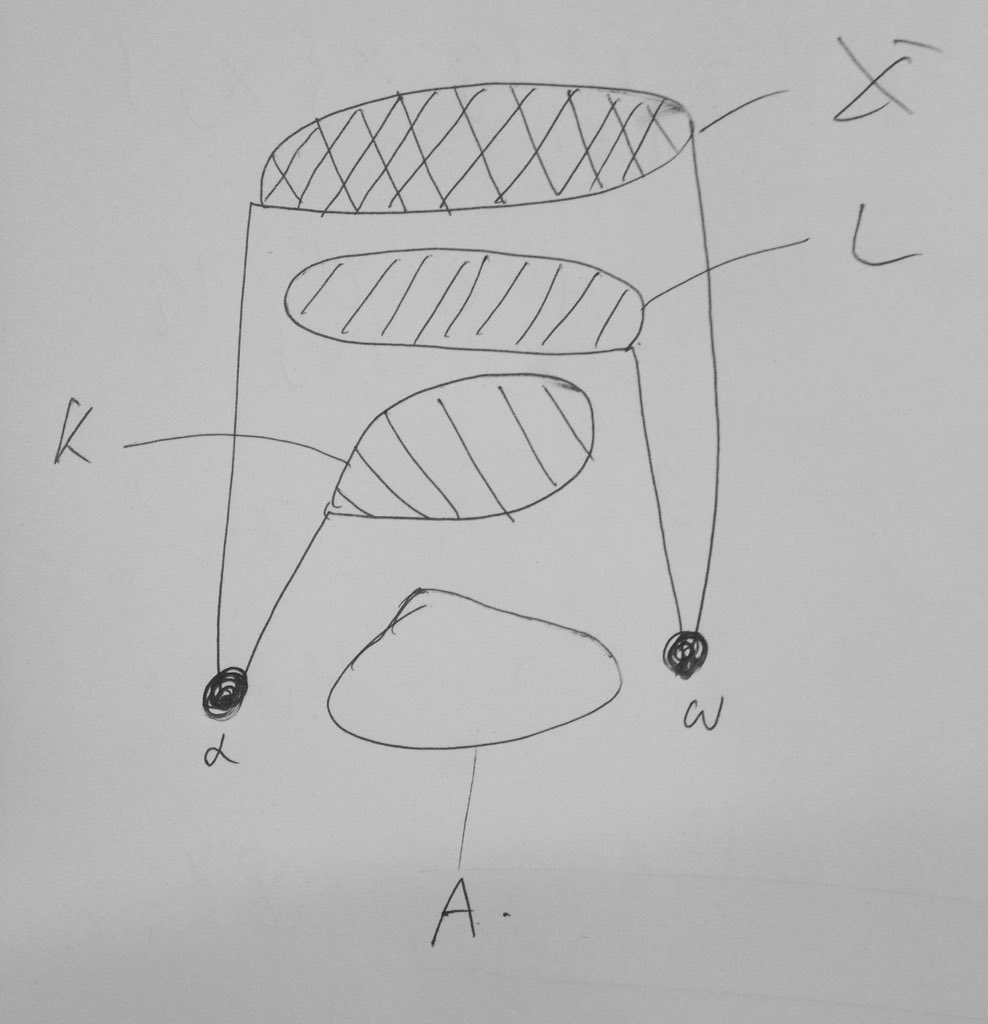
\includegraphics[scale=0.21]{isouX.jpg}
\caption{空間$X$の図}
\end{center}
\end{figure}

















			\end{document}



\begin{comment}
[\bigin \endを使わない方法]

{\prop[aa] aaa}
で
\begin{prop}[aa]
aaa
\end{prop}
と同じ\df \thm \proof でも同様

[直和]
$\amalg$

[同値関係でよく使う波線]
\sim

[引数付きの新命令]
\newcommand{\prn}[1]{\|#1\|_p}

[番号のリセット]

\setcounter{equation}{0}


[字体の変更]

{\rm hogehoge}と使う。

\rm ローマン
\it イタリック
\sl 斜体

[supp]

\newcommand{\supp}{\text{{\rm supp}}}

[中央揃えの改行]

	\begin{eqnarray*}
		hoge1&=&hogehoge
		hoge2&=&hogehofe

	\end{eqnarray*}

&&の部分で揃えられる。






[場合分け]

	\begin{cases}
		hoge1 & \text{状況１}\\
		hoge2 & \text{状況２}\\
		・
		・
		・
	\end{cases}



\end{comment}





